\documentclass{article}

\usepackage[colorlinks=true]{hyperref}
\usepackage{amsmath}
\usepackage{graphicx}
\usepackage{float}
\usepackage{geometry} 
% \usepackage{algorithm}
% \usepackage{algpseudocode}

\begin{document}

\section{Problem Overview}
We can define the problem as a search problem with an agent in answers $w
    \times h$ torus grid world, where the state space is $\mathcal{S}=\{(i, j) |
    \forall i, j: 0 \le i \le w, 0 \le j \le h\}$. Our agent has no knowledge of
the size of the world, nor of which state they are in. The action space is
$\mathcal A = \{up down, left, right\}$ or in terms of our torus $\forall (i,
    j) \in \mathcal S, \mathcal A = \{(i, j + 1 \mod h), (i, j - 1 \mod h), ( i + 1
    \mod w, j), (i + 1 \mod w, j), (i - 1\mod w, j) \}$.

The goal is to reach a goal state, which could be any state on the torus. The
algorithm must always succeed and be linearly bounded by $\mathbf O(35 S)$
where $S = w * h$ or the area of the torus.

Several mathematical properties of our environment and solution must be defined
to proceed. 

We can reformulate the problem as visiting all possible spaces on the torus. This is due to the fact that we have no knowledge of the environment
and the goal can be on any single state. This reformulation also gives us the freedom to also start from an arbitrary location - as the torus wraps around
the starting location is irrelevant for its enu

The goal can be on any spot of the torus and we can start anyhere
on it as well. B to the wrap-around properties of the torus, we can
reforumulate the problem as visiting all possible spaces on the torus (and
enumerating it) rather than visiting a specific goal state. As this is a torus,
our starting state is irrelevant, and we can always start at state $s_0 = (0, 0)$.

\section{Solution}
To be sure all spots on the torus are visited, we must ensure our algorithm never enters a periodic cycle prior to enumerating 
the whole torus. Otherwise, that would leave edge cases with some unenumberated state(s). For example, a simple diagonal policy ($right \to down \to right \to down$) would 
enter a cycle on evenly sized, symmetric grids.

\subsection*{Baseline solution}
The simplest solution with a guarantee of enumerating all states is a simple spiral outward. It only requires knowledge of the initial state and grows outward. In all cases, it would steadily grow in at least 
one axis toward unvisited states, assuring eventually all states are visited (and consequently the goal state). Pseudocode provided in along with a visualization in \autoref{fig:visualization of algorithm}. Unfortunately its runtime comlexity is 
quadratic with respect to the larger side of the grid: $\mathbf O(\max(w, h)^2)$, as the spira will always enumerate a square with sides equal to the larger side. In many cases this violates our 
$O(35S)$ restriction. For example, for $w=1, h = 10^6$, the algorithm would do $10^{12}$ steps or $10^6 * S$ 

\begin{figure}[H]
    \begin{center}
        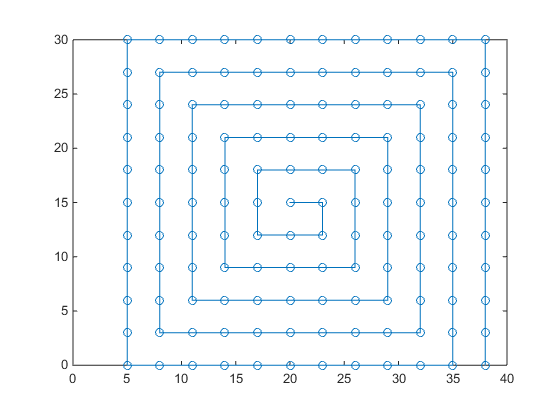
\includegraphics[width=0.4\linewidth]{grid_spiral.png}
        \caption{How the spiral algorithm looks like. It is visible how it grows outward and would eventuall cover the entire grid.Image credit:\url{https://stackoverflow.com/questions/29466058/spiral-loop-on-a-matrix-from-a-point} }
    \end{center}
    \label{fig:visualization of algorithm}
\end{figure}

\section{Time Complexity Analysis}
\section{Alternatives considered}

\end{document}

